\chapter{Kiến trúc và thiết kế hệ thống}
\label{Chapter4}

Chương này trình bày cách nhóm chúng em tổ chức Yoca từ giao diện, máy chủ API đến cơ sở dữ liệu và các nhà cung cấp bên ngoài. Kiến trúc hiện tại không phải là kết quả của một bản thiết kế cố định ngay từ đầu. Nó được điều chỉnh nhiều lần khi nhóm hiểu rõ hơn dữ liệu Solana, giới hạn của các gói API và chi phí duy trì những phép phân tích ví. Vì vậy, nội dung chương tập trung vào những nguyên tắc đang thực sự chi phối mã nguồn, đồng thời chỉ rõ các điểm mà hệ thống vẫn mang dấu vết của quá trình phát triển tăng dần.

\section{Kiến trúc tổng thể}

Yoca là một ứng dụng web full-stack được quản lý trong cùng một monorepo. Phía người dùng sử dụng React và Vite; phía máy chủ là một ứng dụng Hono chạy trên Node.js; dữ liệu có cấu trúc và cache bền vững được lưu trong PostgreSQL thông qua Drizzle ORM. Backend được triển khai như một monolith, nhưng mã nguồn được chia theo miền như token, pool, wallet, người dùng, cảnh báo, thanh toán và AI. Cách tổ chức này vừa đủ nhẹ cho quy mô nhóm, đồng thời tránh chi phí vận hành nhiều dịch vụ độc lập khi các chức năng vẫn chia sẻ lược đồ và dữ liệu.

\begin{figure}[H]
    \centering
    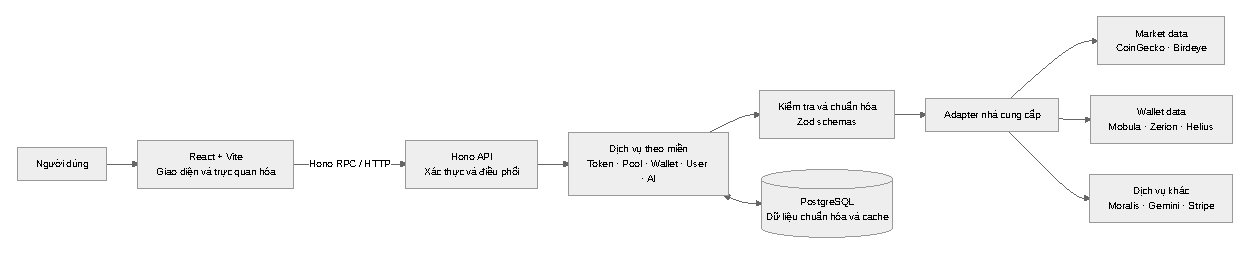
\includegraphics[width=\textwidth]{Chapter4/system-architecture.pdf}
    \caption{Kiến trúc tổng thể của hệ thống Yoca}
    \label{fig:system-architecture}
\end{figure}

Giao diện không gọi trực tiếp API của các nhà cung cấp. Mọi yêu cầu đi qua backend để xác thực, kiểm tra dữ liệu đã lưu, gọi nguồn bên ngoài khi cần và chuyển phản hồi về mô hình nội bộ. Ranh giới này đặc biệt quan trọng vì các provider không chỉ khác tên trường mà còn khác cách biểu diễn token, thời gian, giá trị rỗng và phạm vi lịch sử. Nếu để từng màn hình tự xử lý những khác biệt đó, thay đổi từ một provider sẽ lan sang nhiều thành phần giao diện.

Đây là kiến trúc phân lớp theo trách nhiệm, không phải sự phân tách tuyệt đối. Trong mã nguồn còn tồn tại cả cấu trúc \texttt{routes/services} cũ và một số module mới được gom theo miền. Nhóm chúng em xem đây là kết quả của cách nâng cấp tăng dần: chức năng mới được hoàn thiện và thay thế luồng cũ, sau đó phần không còn được sử dụng mới được loại bỏ. Cách làm này giúp hệ thống tiếp tục hoạt động trong lúc dữ liệu và yêu cầu thay đổi, nhưng cũng tạo ra khoản nợ cần tiếp tục đồng nhất hóa sau đồ án.

\section{Hợp đồng dữ liệu từ giao diện đến nhà cung cấp}

Ứng dụng dùng TypeScript ở cả client và server. Backend xuất kiểu của toàn bộ cây route Hono, còn client khởi tạo RPC client từ chính kiểu đó. Nhờ vậy, đường dẫn, tham số và kiểu phản hồi được kiểm tra ngay trong quá trình phát triển thay vì phải duy trì thêm một bộ khai báo API viết tay. Đây là lý do nhóm chọn Hono: với quy mô hiện tại, Hono RPC tạo được hợp đồng end-to-end mà không cần sinh mã từ một đặc tả trung gian \cite{hono}.

Kiểu TypeScript chỉ tồn tại trong lúc phát triển nên không thể bảo đảm dữ liệu trả về từ Internet là đúng. Trước khi đưa phản hồi của provider vào nghiệp vụ hoặc cơ sở dữ liệu, các service quan trọng sử dụng Zod để kiểm tra cấu trúc ở runtime. Khi một trường sai kiểu, thiếu ngoài dự kiến hoặc mang hình dạng khác tài liệu, hệ thống dừng tại biên tích hợp và trả lỗi thay vì tiếp tục tính toán bằng dữ liệu mơ hồ. Nhóm chúng em chủ ý chọn cách \textit{fail-fast} này vì một kết quả PnL trông hợp lý nhưng được tính từ dữ liệu sai nguy hiểm hơn một yêu cầu thất bại có thể truy vết.

Zod cho phép định nghĩa schema và kiểm tra dữ liệu không đáng tin cậy ngay khi chương trình đang chạy, phù hợp với vai trò bảo vệ biên tích hợp của Yoca \cite{zod}.

Việc kiểm tra chặt cũng làm lộ ra một khó khăn thực tế: tài liệu của provider không phải lúc nào cũng nói rõ trường nào có thể rỗng. Chẳng hạn, địa chỉ token là định danh chắc chắn hơn tên hoặc ký hiệu; các chỉ số biến động giá cũng có thể không tồn tại với token mới hay ít thanh khoản. Lược đồ nội bộ vì vậy không sao chép nguyên xi một phản hồi mẫu, mà chấp nhận giá trị thiếu ở nơi dữ liệu thực tế đòi hỏi và giữ ràng buộc chặt cho các định danh cốt lõi.

Một contract đại diện là API lịch sử cảnh báo. Client gọi \texttt{GET /api/alerts/history} với \texttt{page} và \texttt{limit}; server lấy \texttt{userId} từ phiên xác thực thay vì nhận từ query, nhờ đó người dùng không thể yêu cầu lịch sử của tài khoản khác. Phản hồi gồm danh sách theo thứ tự mới nhất, tổng số bản ghi và số chưa đọc. Mỗi item giữ nguồn cảnh báo, message, severity, trạng thái email/Discord, thời điểm gửi và \texttt{readAt}. Khi cập nhật \texttt{PATCH /api/alerts/history/:id/read}, điều kiện truy vấn đồng thời dùng history ID và user ID; bản ghi không thuộc tài khoản được trả như không tồn tại.

\begin{table}[H]
\centering
\caption{Contract đại diện của API Alert History}
\label{tab:alert-history-contract}
\renewcommand{\arraystretch}{1.15}
\small
\begin{tabularx}{\textwidth}{|p{3.2cm}|X|X|}
\hline
\textbf{Thành phần} & \textbf{Dữ liệu hợp lệ} & \textbf{Hành vi khi không hợp lệ/không đầy đủ} \\
\hline
List history & \texttt{page >= 1}, \texttt{1 <= limit <= 100}; user lấy từ JWT & Query sai trả lỗi validation; lỗi database trả 500; không có dữ liệu trả danh sách rỗng cùng tổng bằng 0 \\
\hline
Read state & UUID history và boolean \texttt{read}; update được scope bởi user & UUID sai trả 400; ID không tồn tại hoặc thuộc user khác trả 404 \\
\hline
Delivery snapshot & Ít nhất một kênh gửi thành công; lưu attempted/succeeded riêng cho email và Discord & Partial delivery vẫn được lưu đúng trạng thái từng kênh; không kênh nào thành công thì không tạo history \\
\hline
Idempotency & Khóa logic từ user, transaction signature, scope và rule/ví & Webhook retry cùng sự kiện không tạo bản ghi thứ hai \\
\hline
\end{tabularx}
\end{table}

\section{Luồng truy xuất, chuẩn hóa và lưu đệm}

Mẫu truy xuất phổ biến trong backend gồm hai lớp hàm. Hàm \texttt{get*} là điểm vào của route: nó tìm dữ liệu trong cơ sở dữ liệu và đánh giá độ mới. Nếu dữ liệu còn hợp lệ, kết quả được trả ngay; nếu thiếu hoặc đã cũ, hàm gọi luồng \texttt{fetch*}. Luồng thứ hai chịu trách nhiệm truy cập provider, kiểm tra phản hồi, cập nhật cơ sở dữ liệu rồi trả về cùng kiểu dữ liệu nội bộ. Không phải mọi service đều tuân theo đúng tên gọi này, nhưng đây là nguyên tắc chủ đạo đối với dữ liệu thị trường và dữ liệu ví.

Nhóm chúng em không áp dụng fallback nhiều provider một cách mặc định. Mỗi provider được chọn theo phần dữ liệu mà họ có thế mạnh và theo hạn mức còn khả dụng. Token metadata là một trong những nơi cần nhiều nguồn bổ sung, trong khi PnL và lịch sử giao dịch ví hiện dựa chủ yếu vào Mobula; lịch sử tổng tài sản ưu tiên Mobula, còn chuỗi số dư theo từng token tiếp tục dùng Zerion. Helius vẫn giữ vai trò đối với giao dịch on-chain và webhook. Sự phân công theo miền làm giảm số nhánh khó kiểm soát, dù đồng nghĩa hệ thống vẫn phụ thuộc đáng kể vào chất lượng của từng nguồn.

Cơ sở dữ liệu vừa lưu dữ liệu nghiệp vụ, vừa là lớp cache bền vững. Thiết kế bảng không chỉ theo mục tiêu chuẩn hóa mà còn cân nhắc số lần gọi API để hoàn thiện một bản ghi. Nếu một hàng yêu cầu hai hoặc ba endpoint khác nhau nhưng các phần dữ liệu có chu kỳ cập nhật khác nhau, việc tách chúng thành các bảng nhỏ giúp chỉ làm mới phần đã cũ. Khi provider trả kèm thông tin hữu ích, service có thể cập nhật thêm bảng liên quan để tận dụng dữ liệu đã trả phí truy vấn, song việc cập nhật chéo phải đi qua khóa và ràng buộc nhất quán.

\section{Thiết kế cơ sở dữ liệu}
\label{sec:thiet_ke_csdl}

\subsection{Mục tiêu và đặc điểm dữ liệu}
\label{subsec:db_muc_tieu}

Cơ sở dữ liệu PostgreSQL của Yoca được thiết kế theo hai lớp có mục đích khác nhau. Lớp thứ nhất là dữ liệu nền tương đối chuẩn hóa, gồm tài khoản, phương thức xác thực, watchlist, nhãn ví, cảnh báo, subscription và thanh toán. Đây là dữ liệu do người dùng hoặc hệ thống sở hữu, cần khóa ngoại và quy tắc xóa rõ ràng. Lớp thứ hai là các read model và cache bền vững cho token, pool, ví, giao dịch và kết quả phân tích. Lớp này ưu tiên khả năng đọc nhanh, tái sử dụng dữ liệu provider và làm mới từng phần hơn là loại bỏ mọi sự lặp dữ liệu.

Dữ liệu trong Yoca có hai đặc điểm. Dữ liệu tài khoản và thanh toán cần quan hệ rõ ràng, ràng buộc khóa ngoại và quy tắc xóa nhất quán. Ngược lại, phần lớn dữ liệu blockchain là dữ liệu công khai được định danh bằng token address, wallet address hoặc transaction signature. Các bảng này thường không phụ thuộc vào một bảng gốc duy nhất mà được liên kết theo khóa nghiệp vụ.

Schema được định nghĩa bằng Drizzle ORM. Kiểu dữ liệu, primary key, unique constraint và foreign key được đặt trong mã TypeScript, giúp truy vấn backend và cấu trúc PostgreSQL dùng chung một định nghĩa. Tuy nhiên, schema vật lý không phải lúc nào cũng trùng với mô hình khái niệm: wallet address, token address và signature thường là khóa nghiệp vụ liên kết nhiều bảng nhưng không bị buộc phải tham chiếu đến một bảng cha.

\subsection{Phân nhóm dữ liệu theo miền nghiệp vụ}
\label{subsec:db_phan_nhom}

Cấu trúc lưu trữ được chia theo các miền identity/payment, token/market, wallet/analysis, transaction, alert và content/AI. Hình~\ref{fig:db_overview} chỉ thể hiện quan hệ khái niệm giữa các miền; các ERD phía sau mới phân biệt foreign key vật lý với liên hệ bằng address hoặc signature.

\begin{figure}[H]
    \centering
    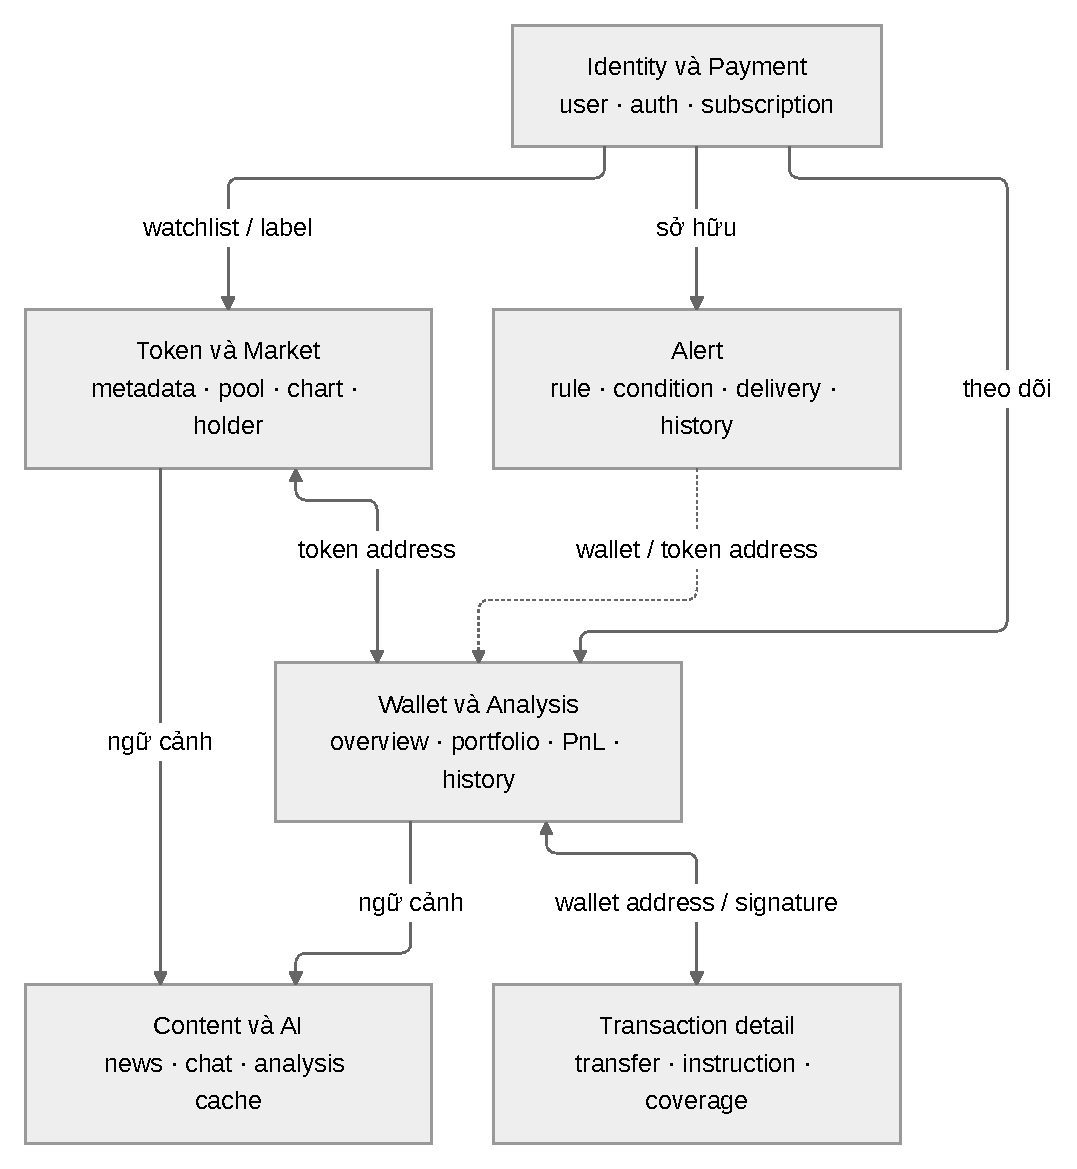
\includegraphics[width=0.9\textwidth,height=0.68\textheight,keepaspectratio]{Chapter3/diagrams/database-overview.pdf}
    \caption{Các miền dữ liệu chính và quan hệ khái niệm}
    \label{fig:db_overview}
\end{figure}

Các nhóm trên phục vụ nhu cầu truy vấn khác nhau. Vì vậy, dữ liệu có thể giao nhau về wallet address, token address hoặc transaction signature nhưng không đồng nghĩa các bảng có thể thay thế trực tiếp cho nhau. Cách phân nhóm cũng giúp ERD tổng thể không biến thành một hình quá dài theo chiều ngang và phải thu nhỏ đến mức không đọc được.

\subsection{Sơ đồ thực thể mối quan hệ}
\label{subsec:db_erd}

Schema có nhiều bảng cache nên một ERD duy nhất sẽ khó đọc trên khổ A4. Phần này chia ERD theo miền nghiệp vụ và chỉ giữ primary key, foreign key cùng các cột chính. Đường liền biểu diễn foreign key được khai báo trong PostgreSQL. Đường nét đứt biểu diễn liên hệ logic thông qua address, mint hoặc signature; các liên hệ này được kiểm soát tại service thay vì bằng foreign key.

\begin{figure}[H]
    \centering
    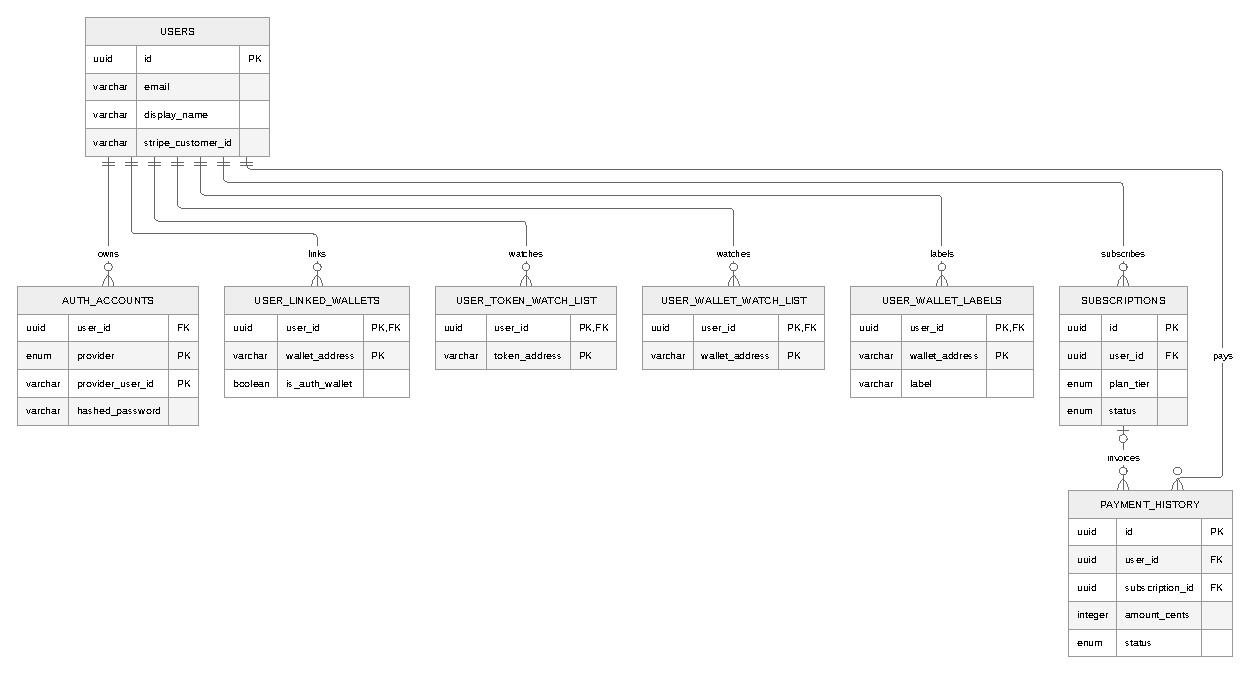
\includegraphics[width=\textwidth,height=0.78\textheight,keepaspectratio]{Chapter3/diagrams/identity-payment.pdf}
    \caption{ERD nhóm tài khoản và thanh toán}
    \label{fig:db_identity_payment}
\end{figure}

Hình~\ref{fig:db_identity_payment} thể hiện dữ liệu có tính sở hữu. Bảng \texttt{users} là gốc của dữ liệu xác thực, cấu hình cá nhân và thanh toán. Các bản ghi phụ thuộc người dùng được xóa theo quan hệ cascade; lịch sử thanh toán giữ được bản ghi khi subscription không còn tồn tại.

\begin{figure}[H]
    \centering
    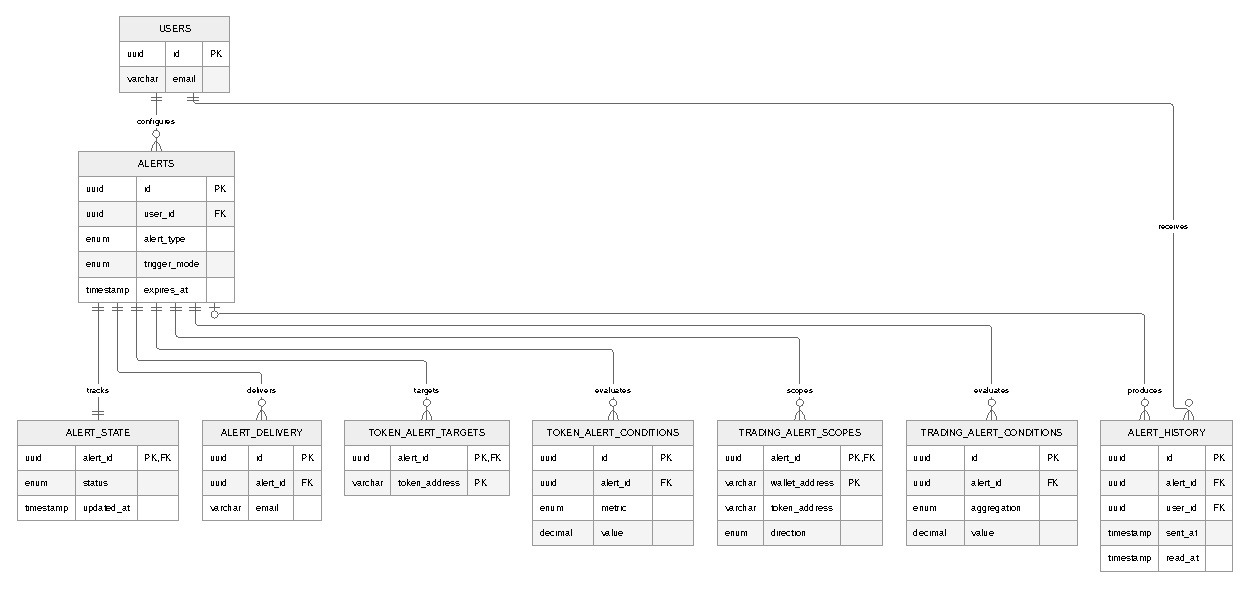
\includegraphics[width=\textwidth,height=0.78\textheight,keepaspectratio]{Chapter3/diagrams/alert-history.pdf}
    \caption{ERD nhóm cảnh báo và lịch sử cảnh báo}
    \label{fig:db_alert_history}
\end{figure}

Hình~\ref{fig:db_alert_history} tách định nghĩa cảnh báo khỏi trạng thái, delivery target và điều kiện kích hoạt. \texttt{alert\_history} lưu sự kiện đã phát sinh để hỗ trợ hiển thị lịch sử và trạng thái đã đọc.

\begin{figure}[H]
    \centering
    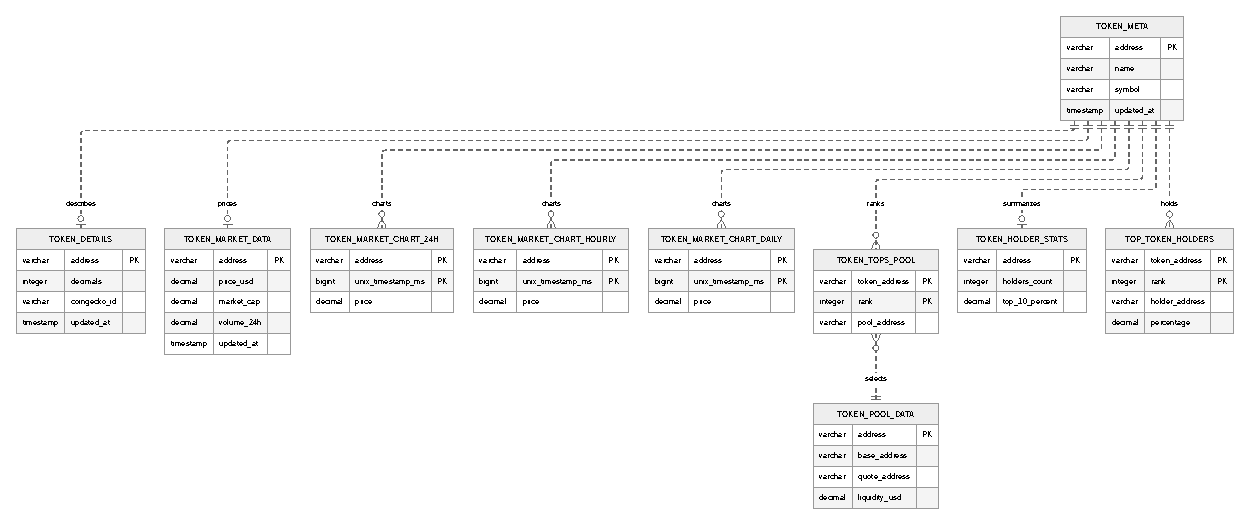
\includegraphics[width=\textwidth,height=0.78\textheight,keepaspectratio]{Chapter3/diagrams/token-market.pdf}
    \caption{ERD nhóm token và dữ liệu thị trường}
    \label{fig:db_token_market}
\end{figure}

Hình~\ref{fig:db_token_market} sử dụng \texttt{token\_meta} như điểm tham chiếu logic. Market snapshot và chart được cập nhật theo address và mốc thời gian. Pool và holder là các read model riêng, chỉ liên kết logic với token.

\begin{figure}[H]
    \centering
    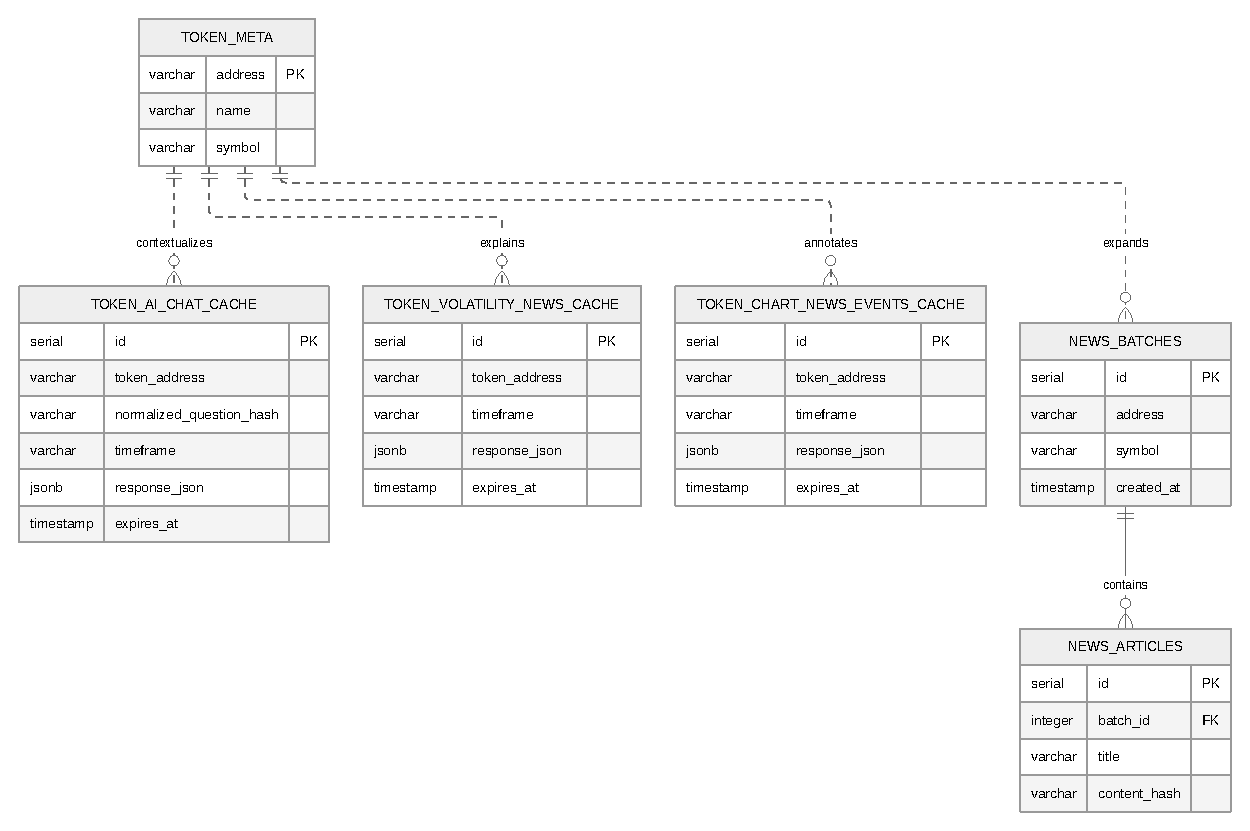
\includegraphics[width=\textwidth,height=0.78\textheight,keepaspectratio]{Chapter3/diagrams/token-content.pdf}
    \caption{ERD nhóm nội dung và AI cache theo token}
    \label{fig:db_token_content}
\end{figure}

Hình~\ref{fig:db_token_content} mô tả các cache phục vụ AI, news event và phần giải thích biến động. News batch có quan hệ khóa ngoại trực tiếp với article; các cache còn lại được ghép với token theo address.

\begin{figure}[H]
    \centering
    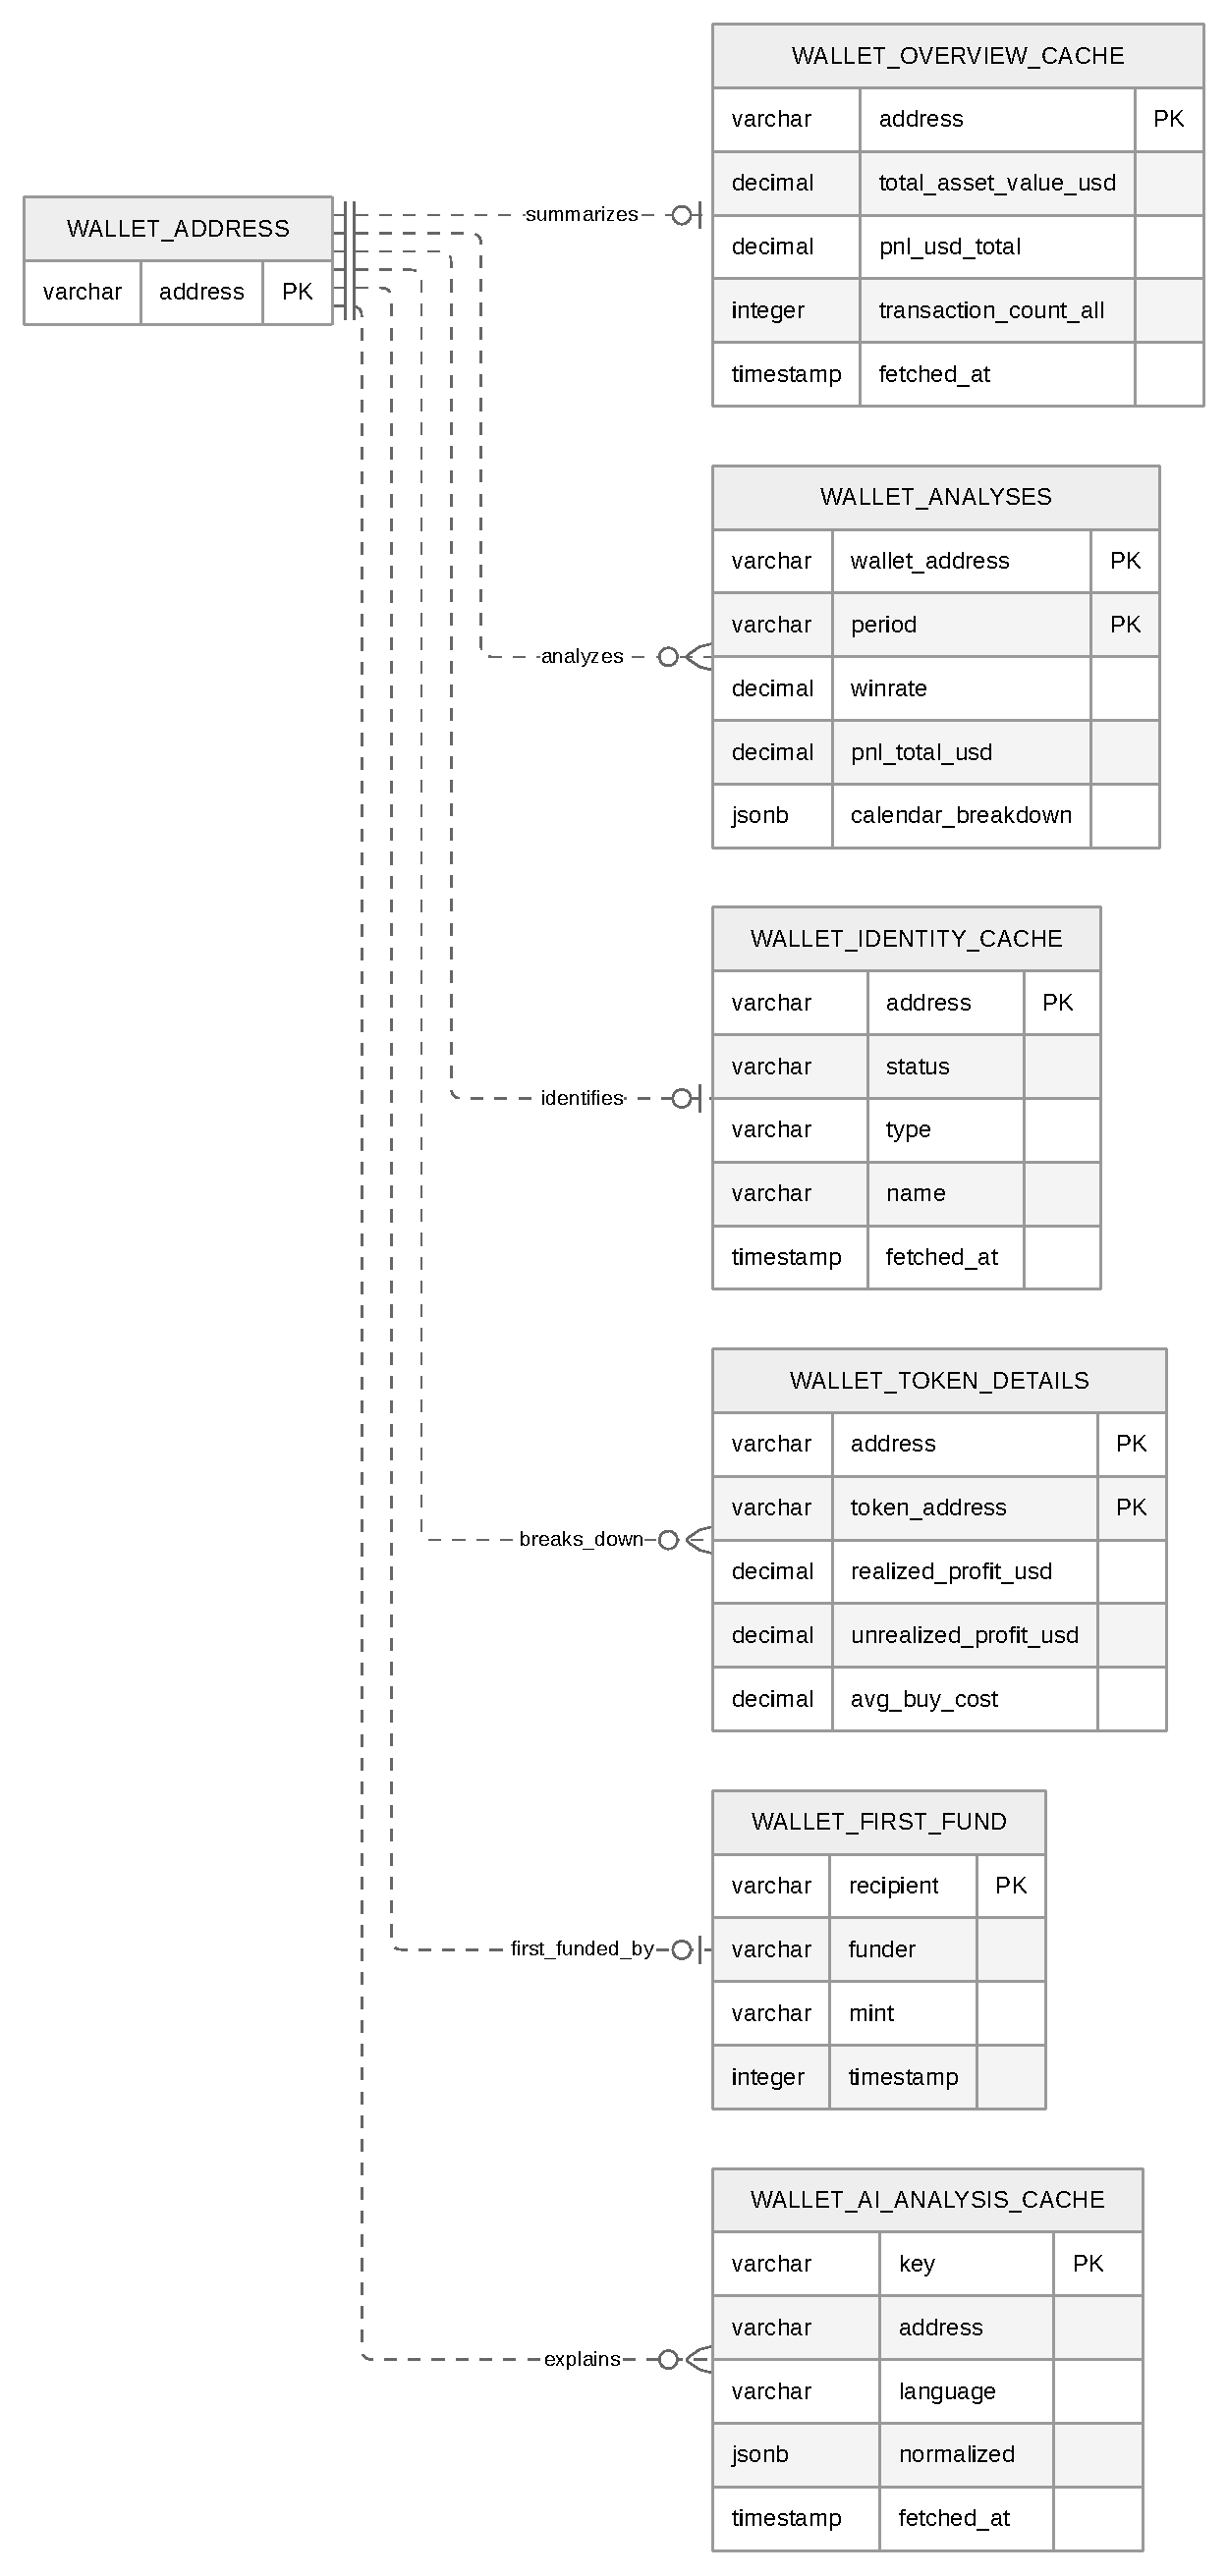
\includegraphics[width=\textwidth,height=0.78\textheight,keepaspectratio]{Chapter3/diagrams/wallet-analytics.pdf}
    \caption{ERD nhóm tổng quan và phân tích ví}
    \label{fig:db_wallet_analytics}
\end{figure}

Hình~\ref{fig:db_wallet_analytics} dùng \texttt{WALLET\_ADDRESS} như một thực thể logic, không phải bảng vật lý. \texttt{wallet\_overview\_cache} cung cấp bản tổng hợp cho trang overview. \texttt{wallet\_analyses} lưu kết quả Mobula theo ví và kỳ phân tích.

\begin{figure}[H]
    \centering
    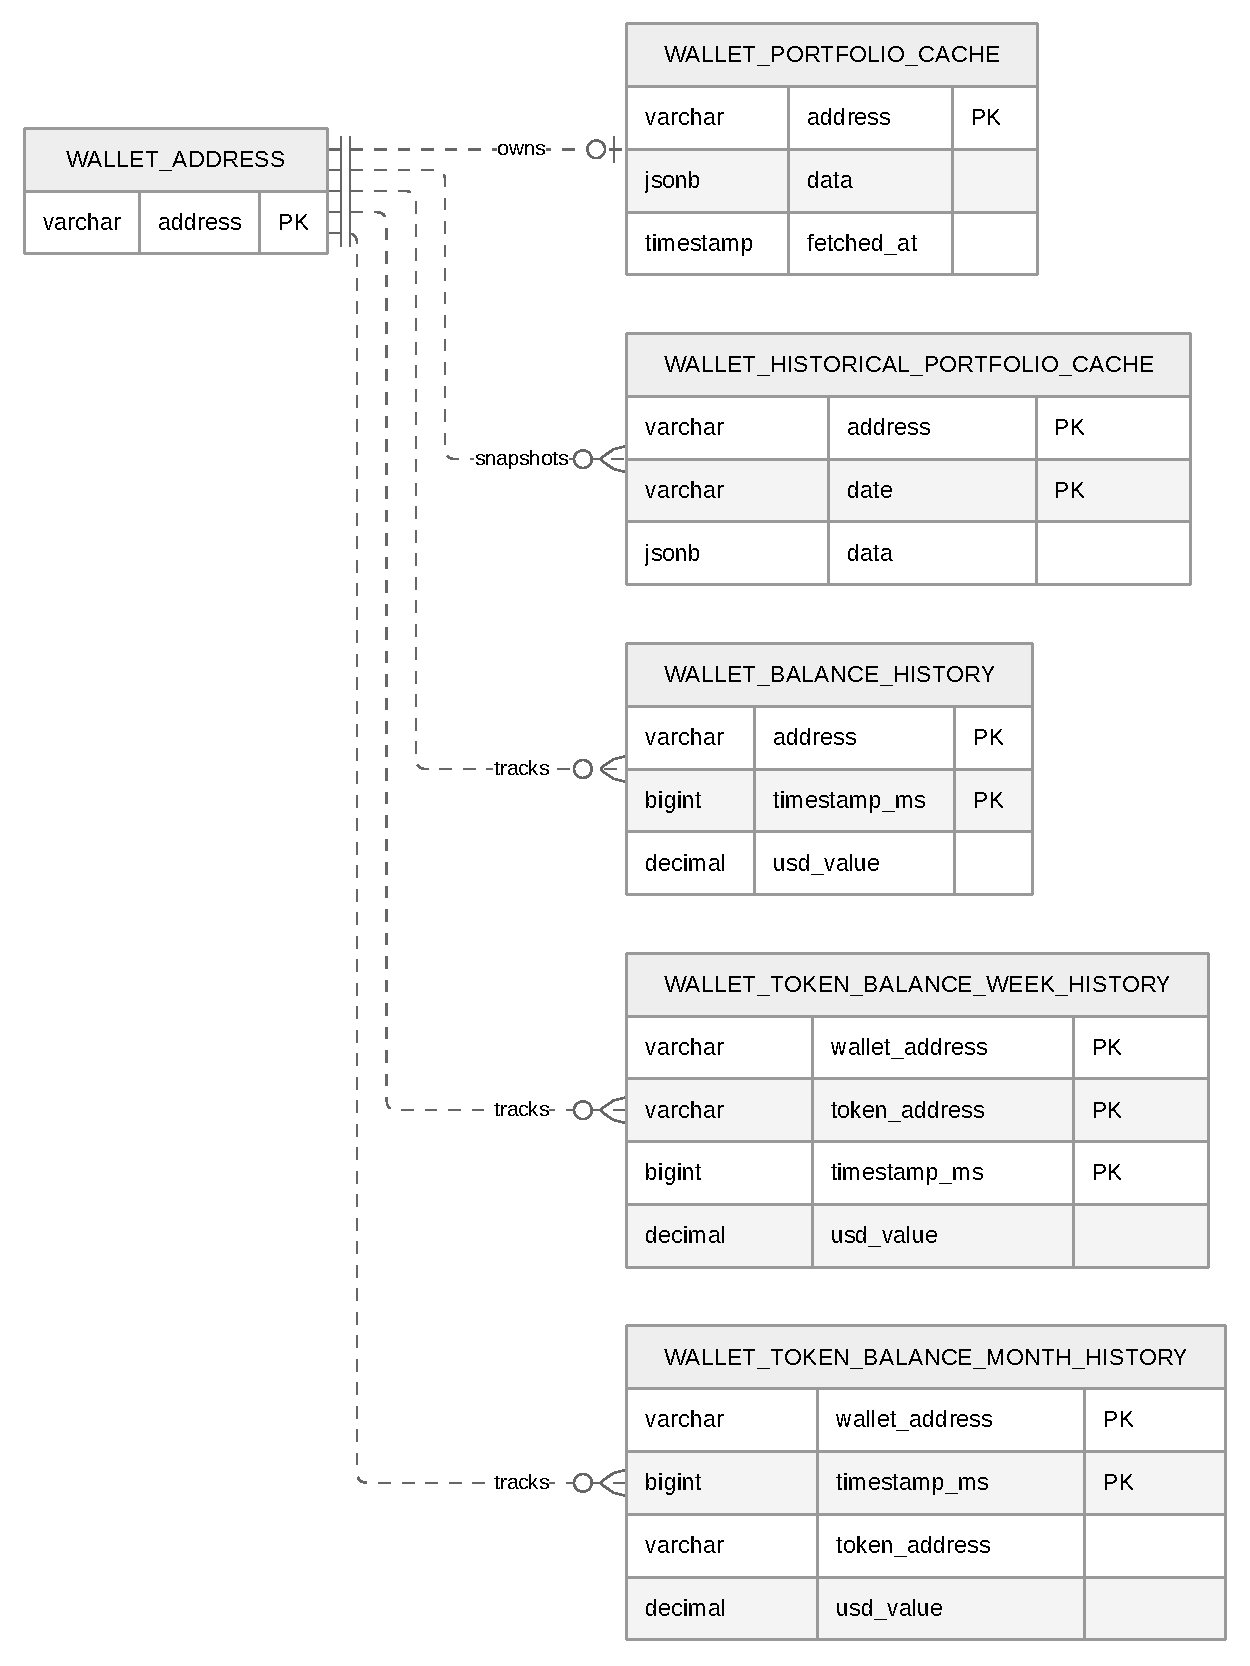
\includegraphics[width=\textwidth,height=0.78\textheight,keepaspectratio]{Chapter3/diagrams/wallet-portfolio-balance.pdf}
    \caption{ERD nhóm portfolio và lịch sử số dư}
    \label{fig:db_wallet_portfolio_balance}
\end{figure}

Hình~\ref{fig:db_wallet_portfolio_balance} phân biệt portfolio hiện tại, snapshot theo ngày, tổng giá trị ví theo thời gian và lịch sử số dư ở cấp token. Các bảng được ghép theo wallet address nhưng không phụ thuộc một bảng wallet vật lý.

\begin{figure}[H]
    \centering
    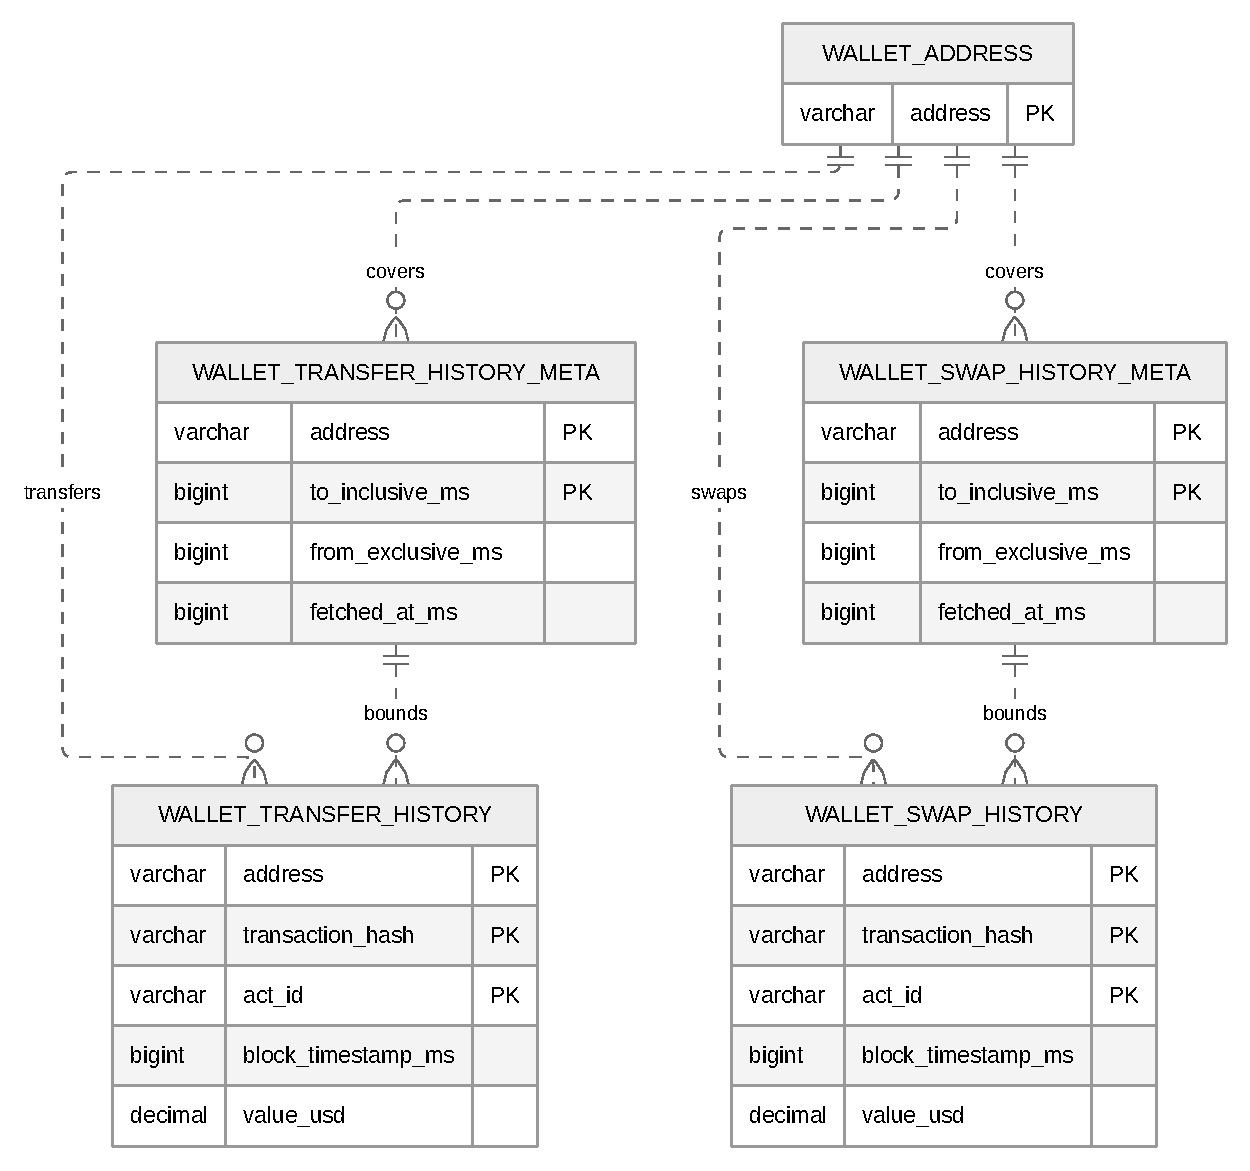
\includegraphics[width=\textwidth,height=0.78\textheight,keepaspectratio]{Chapter3/diagrams/wallet-history.pdf}
    \caption{ERD nhóm lịch sử transfer và swap}
    \label{fig:db_wallet_history}
\end{figure}

Hình~\ref{fig:db_wallet_history} tách dữ liệu lịch sử đã chuẩn hóa khỏi metadata coverage. Các bảng này phục vụ truy vấn phân trang và chỉ tải bổ sung những khoảng thời gian còn thiếu.

\begin{figure}[H]
    \centering
    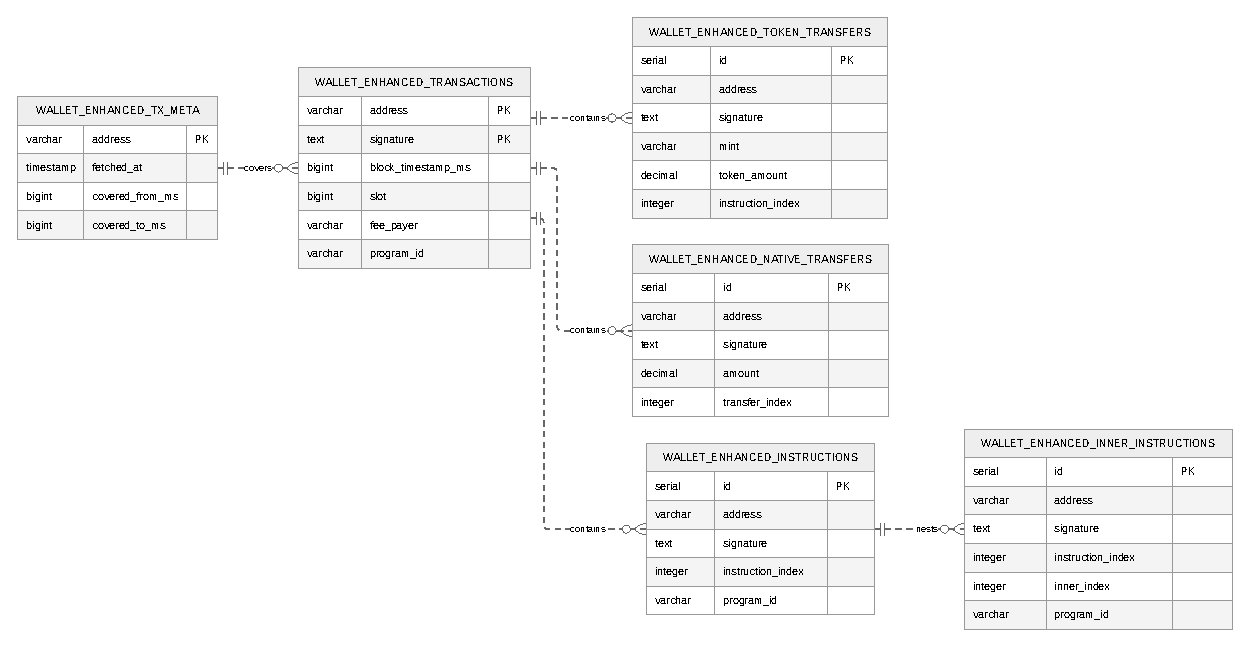
\includegraphics[width=\textwidth,height=0.78\textheight,keepaspectratio]{Chapter3/diagrams/enhanced-transaction-detail.pdf}
    \caption{ERD nhóm chi tiết giao dịch Helius}
    \label{fig:db_enhanced_transaction_detail}
\end{figure}

Hình~\ref{fig:db_enhanced_transaction_detail} mô tả read model chi tiết giao dịch. Bảng transaction cha được ghép với token transfer, native transfer và instruction bằng address cùng signature. Nhóm này phục vụ day activity, transaction detail và wallet analysis; nó không bị thay thế bởi transfer/swap history.

\subsection{Các bảng trọng tâm}
\label{subsec:db_bang_trong_tam}

Bảng~\ref{tab:db_core_tables} tóm tắt các bảng đại diện cho từng miền. Các bảng cache phụ có cùng cách tổ chức không được liệt kê lại để tránh lặp nội dung.

\begin{longtable}{|L{0.27\textwidth}|L{0.25\textwidth}|L{0.38\textwidth}|}
\caption{Các bảng dữ liệu trọng tâm của Yoca}
\label{tab:db_core_tables}\\
\hline
\textbf{Bảng} & \textbf{Khóa chính} & \textbf{Vai trò} \\
\hline
\endfirsthead
\hline
\textbf{Bảng} & \textbf{Khóa chính} & \textbf{Vai trò} \\
\hline
\endhead
\texttt{users} & \texttt{id} & Thông tin tài khoản, cấu hình nhận cảnh báo và Stripe customer. \\
\hline
\texttt{auth\_accounts} & \texttt{provider, provider\_user\_id} & Danh tính đăng nhập bằng password, OAuth hoặc ví Solana. \\
\hline
\texttt{subscriptions} & \texttt{id} & Trạng thái gói dịch vụ và chu kỳ thanh toán. \\
\hline
\texttt{alerts} & \texttt{id} & Định nghĩa cảnh báo, loại cảnh báo, chế độ kích hoạt và thời hạn. \\
\hline
\texttt{alert\_history} & \texttt{id} & Lịch sử cảnh báo đã phát sinh và trạng thái đã đọc. \\
\hline
\texttt{token\_meta} & \texttt{address} & Tên, symbol và hình ảnh cơ bản của token. \\
\hline
\texttt{token\_market\_data} & \texttt{address} & Market snapshot gần nhất, gồm giá, vốn hóa và volume. \\
\hline
\texttt{token\_market\_chart\_*} & \texttt{address, timestamp} & Chuỗi giá 24 giờ, hourly và daily cho biểu đồ. \\
\hline
\texttt{wallet\_overview\_cache} & \texttt{address} & Read model tổng hợp tài sản, volume, PnL và hoạt động của ví. \\
\hline
\texttt{wallet\_analyses} & \texttt{wallet\_address, period} & Kết quả Mobula gồm win rate, PnL, phân phối giao dịch và calendar breakdown. \\
\hline
\texttt{wallet\_transfer\_history} & \texttt{address, transaction\_hash, act\_id} & Lịch sử chuyển token đã chuẩn hóa và hỗ trợ phân trang. \\
\hline
\texttt{wallet\_swap\_history} & \texttt{address, transaction\_hash, act\_id} & Lịch sử swap đã chuẩn hóa theo ví. \\
\hline
\texttt{wallet\_enhanced\_transactions} & \texttt{address, signature} & Transaction cha cho dữ liệu chi tiết từ Helius. \\
\hline
\texttt{chat\_sessions} & \texttt{id} & Phiên chat, context ví và danh sách message. \\
\hline
\texttt{news\_batches} & \texttt{id} & Nhóm bài viết thu thập theo token và thời điểm. \\
\hline
\end{longtable}

\texttt{wallet\_analyses} là read model có kích thước tương đối lớn do lưu cả chỉ số tổng hợp và hai cấu trúc JSONB là \texttt{period\_timeframes} và \texttt{calendar\_breakdown}. Mỗi ví chỉ có một bản ghi cho mỗi kỳ phân tích, nhờ đó dữ liệu Mobula có thể được dùng lại trong thời gian TTL mà không cần gọi provider cho mọi request.

Các bảng \texttt{wallet\_enhanced\_*} lưu chi tiết giao dịch ở mức thấp hơn transfer/swap history. Instruction, inner instruction, fee payer, program ID và native transfer cần thiết cho transaction detail và phân tích hành vi, trong khi history tables ưu tiên danh sách đã chuẩn hóa và phân trang.

\subsection{Cache và quản lý độ mới}
\label{subsec:db_cache}

Cache được kiểm soát bằng ba cơ chế. Cơ chế thứ nhất là TTL dựa trên thời điểm cập nhật. Dữ liệu overview, market hoặc kết quả phân tích được trả trực tiếp khi vẫn còn mới; khi hết TTL, service gọi provider và cập nhật lại bản ghi.

Cơ chế thứ hai là coverage metadata. Với lịch sử ví và enhanced transaction, metadata lưu khoảng thời gian đã đồng bộ. Service so sánh khoảng yêu cầu với khoảng đã có, chỉ tải phần còn thiếu rồi hợp nhất coverage. Cách này tránh tải lại toàn bộ lịch sử của ví.

Cơ chế thứ ba là upsert. Market snapshot, chart point và các cache theo khóa nghiệp vụ sử dụng insert kết hợp conflict handling. Bản ghi mới được thêm khi khóa chưa tồn tại; dữ liệu cũ được cập nhật khi cùng address, timestamp hoặc signature.

\subsection{Toàn vẹn và bảo mật dữ liệu}
\label{subsec:db_toan_ven}

Primary key tổng hợp được dùng cho dữ liệu chuỗi thời gian và lịch sử, ví dụ address kết hợp timestamp hoặc transaction hash. Unique constraint ngăn một transaction detail hoặc chart point bị ghi nhiều lần. Foreign key với quy tắc cascade áp dụng cho dữ liệu thuộc người dùng như auth account, watchlist, alert và subscription.

Không phải mọi liên hệ logic đều được chuyển thành foreign key. Wallet address và token address đến từ blockchain, có thể xuất hiện trước khi metadata tương ứng được tải. Việc bắt buộc foreign key trong trường hợp này sẽ làm gián đoạn luồng đồng bộ. Service chịu trách nhiệm chuẩn hóa address và giữ quy tắc ghép dữ liệu nhất quán.

Dữ liệu công khai từ blockchain được tách khỏi dữ liệu cá nhân. Các truy vấn profile, watchlist, cảnh báo, chat và thanh toán phải được giới hạn theo user ID đã xác thực. Password chỉ được lưu dưới dạng hash; API key và secret của provider không được lưu trong các bảng nghiệp vụ.

% TODO(runtime): Hoàn thiện ghi alert_history sau khi delivery thành công.
% TODO(runtime): Bổ sung API lấy lịch sử, đánh dấu đã đọc và chống gửi trùng.

\subsection{Tổng kết thiết kế cơ sở dữ liệu}
\label{subsec:db_tong_ket}

Thiết kế cơ sở dữ liệu kết hợp dữ liệu quan hệ với các read model cache theo miền nghiệp vụ. Các bảng user, payment và alert ưu tiên ràng buộc quan hệ. Các bảng token và wallet ưu tiên khả năng đồng bộ, truy vấn theo address và tái sử dụng dữ liệu provider. Việc tách overview, history, analysis và transaction detail giúp mỗi endpoint đọc đúng cấu trúc cần thiết thay vì phụ thuộc vào một bảng giao dịch chung.



\section{Lựa chọn công nghệ và giới hạn của thiết kế}

React được chọn vì mô hình thành phần phù hợp với giao diện có nhiều bảng, biểu đồ và trạng thái tương tác dùng lại; Vite cung cấp máy chủ phát triển và cơ chế cập nhật mô-đun nhanh \cite{react,vite}. ECharts đảm nhiệm phần lớn biểu đồ tài chính \cite{echarts}, trong khi các cấu trúc quan hệ giao dịch cần một thành phần đồ thị tương tác riêng. Ở backend, Drizzle được chọn vì cách khai báo lược đồ gần với SQL và cho phép nhóm kiểm soát trực tiếp truy vấn, điều quan trọng khi cache và dữ liệu lịch sử cần các thao tác upsert hoặc truy vấn theo khoảng \cite{drizzle}.

Những lựa chọn trên ưu tiên tốc độ phát triển và khả năng nhìn thấy lỗi sớm, nhưng không tự động tạo ra một hệ thống hoàn toàn nhất quán. Hono RPC chỉ bảo vệ hợp đồng giữa client và server; Zod bảo vệ dữ liệu ở runtime; ràng buộc cơ sở dữ liệu bảo vệ trạng thái đã lưu; còn kiểm thử vẫn cần thiết để xác nhận hành vi kết hợp giữa các lớp. Việc phân biệt các lớp bảo vệ này giúp nhóm không xem ``strongly typed'' như một sự thay thế cho kiểm thử.

Ở phía giao diện, Carbon Design System từng được chọn làm nền tảng chung, nhưng việc hiện thực không được duy trì đồng đều trong suốt quá trình phát triển. Một số màn hình mới kết hợp thành phần tự xây dựng, SCSS và utility class, trong khi một số bảng cũ vẫn giữ cấu trúc Carbon. Nhóm chúng em chấp nhận trình bày đây là hạn chế về tính nhất quán và khả năng bảo trì, thay vì mô tả giao diện như một design system đã hoàn thiện. Trong đợt hoàn thiện cuối, nhóm ưu tiên đồng nhất các luồng chính; những bảng cũ chưa chuyển đổi hoàn toàn được ghi nhận rõ như một giới hạn của phiên bản hiện tại.

Localization được tổ chức thành một lớp dùng chung độc lập với từng trang. Locale tiếng Anh đóng vai trò cấu trúc gốc; locale tiếng Việt phải giữ cùng hệ thống key và biến nội suy. Kiểu TypeScript được dùng để phát hiện key thiếu, key sai và biến interpolation không tương thích trong lúc phát triển. Hook \texttt{useLocalization} cung cấp đồng thời hàm dịch và formatter cho số, phần trăm, token unit, ngày giờ và tiền tệ. Các formatter nhận giá trị tài chính gốc bằng USD; với locale Việt Nam, lớp hiển thị áp dụng tỷ giá USD--VND rồi định dạng theo quy ước VND. Cách tách này giữ phép tính và API ở một đơn vị thống nhất, đồng thời tránh mỗi component tự quy đổi theo một công thức khác nhau.

\section{Kết chương}

Chương 4 đã xác định Yoca là một monolith phân lớp theo miền, có hợp đồng kiểu xuyên suốt giữa client và server, biên kiểm tra runtime cho dữ liệu bên ngoài, cùng cơ chế lưu trữ ưu tiên tái sử dụng dữ liệu đã đồng bộ. Kiến trúc này phản ánh sự cân bằng giữa lược đồ chuẩn hóa, hạn mức API và khả năng phát triển của nhóm. Trên nền thiết kế đó, Chương 5 trình bày kết quả triển khai, những khó khăn đã gặp và mức độ đáp ứng của hệ thống.
